\chapter{ボタン押し課題のシステム}
本章では,遅延聴覚フィードバックが身体運動に与える影響を客観的に評価するための調査で行うボタン押し課題,この調査を行うために構築した調査システム及びWindowsアプリケーションについて述べる.
聴覚フィードバックは遅延時間が大きくなると,発話だけでなく身体運動に影響を与えることが知られている\cite{timing-music}\cite{shimada-DAF}.
身体運動を遅延聴覚フィードバックが与える影響の調査に使用することが可能となれば,客観的なデータを計測しやすくなることが期待される.

\section{ボタン押し課題}
本研究で行う客観評価による調査では,被験者が行う課題にボタン押し課題を採用する.
この調査で採用するボタン押し課題は,ボタンを押下するときの音に遅延を発生させて被験者に聞かせながら,
被験者がメトロノームの合図音に合わせて一定の時間間隔でボタンを押下する課題を行うというものである.
このボタン押し課題は,楽器演奏のような特別な技能を必要としないため,遅延聴覚フィードバックが身体運動に与える影響を様々な年代の被験者について調査することが可能になると考えられる.
ボタン押し課題を行っているとき,被験者がボタンを押下する時間間隔を記録すると,被験者に提示するボタン押下の時間間隔が毎分60回であれば,理想的に全てのボタンを押下する時間間隔が1000[ms]となるが,人間の操作には誤差が生じる.
また,遅延聴覚フィードバックが身体運動に影響を与えていれば,このばらつきを提示するボタンを押下する音の遅延時間によって変化するものであると考えられる.
そのため,遅延聴覚フィードバックを与えている状態で被験者がボタン押し課題を行うと,ボタンを押下する時間間隔に変化が現れることが期待される.
したがって,遅延聴覚フィードバックの下で被験者がボタン押し課題を行うときのボタンを押下する時間間隔を,
様々な遅延時間で観察することで遅延聴覚フィードバックが身体運動に与える影響を客観的に評価することができると考えられる.
この調査で使用するシステムの図を図\ref{fig:button-click-system}に示し,使用機器を表\ref{table:device}に示す.
このシステムは表\ref{table:device}の使用機器と遅延聴覚フィードバックを生成する音響信号への遅延生成アプリケーション,
メトロノーム,研究室で開発したパルスジェネレーターで構成されている.
このパルスジェネレーターは,図\ref{fig:super_famicom}に示したコントローラーのボタンが押下されると,
オペアンプを通じて音響信号がアナログ出力され,オーディオインターフェースにディジタル入力された後,オーディオインターフェースへの信号の入力を合図に,
クリック音がヘッドホンから出力されるという仕組みとなっている.
音響信号への遅延生成アプリケーションは,4.2節で述べられるものと同様である.
以下に,本研究で用いるボタン押し課題の手順と図\ref{fig:button-click-system}のシステムの動作について説明する.
\vskip.5\baselineskip
\begin{enumerate}[leftmargin=*]
\item 被験者はヘッドホンを装着し,コントローラーを手に持つ.コントローラーのA, B, C, Dいずれかのボタンを押すと,任意の遅延時間が経過した後にヘッドホンに「ピッ」というクリック音が出力される.
\item 電子メトロノームの合図音によって,一定間隔でボタンを押下するための合図を提示し,その合図に合わせて,被験者はボタン押し課題を実施する.
ボタン押し課題で被験者がボタンを押下する回数は,アプリケーション上で実験者が設定する.
課題中,PCに保存されたWAVファイルがオーディオインターフェースを介して,実験者が指定した時間だけ遅延してヘッドホンから出力される.
この時,実験者が指定した遅延時間は被験者には非公開とする.また,音響信号への遅延生成アプリケーションは,被験者がボタンを押下する時間間隔の記録も行う.
\end{enumerate}
\begin{figure}[tb]
  \centering
  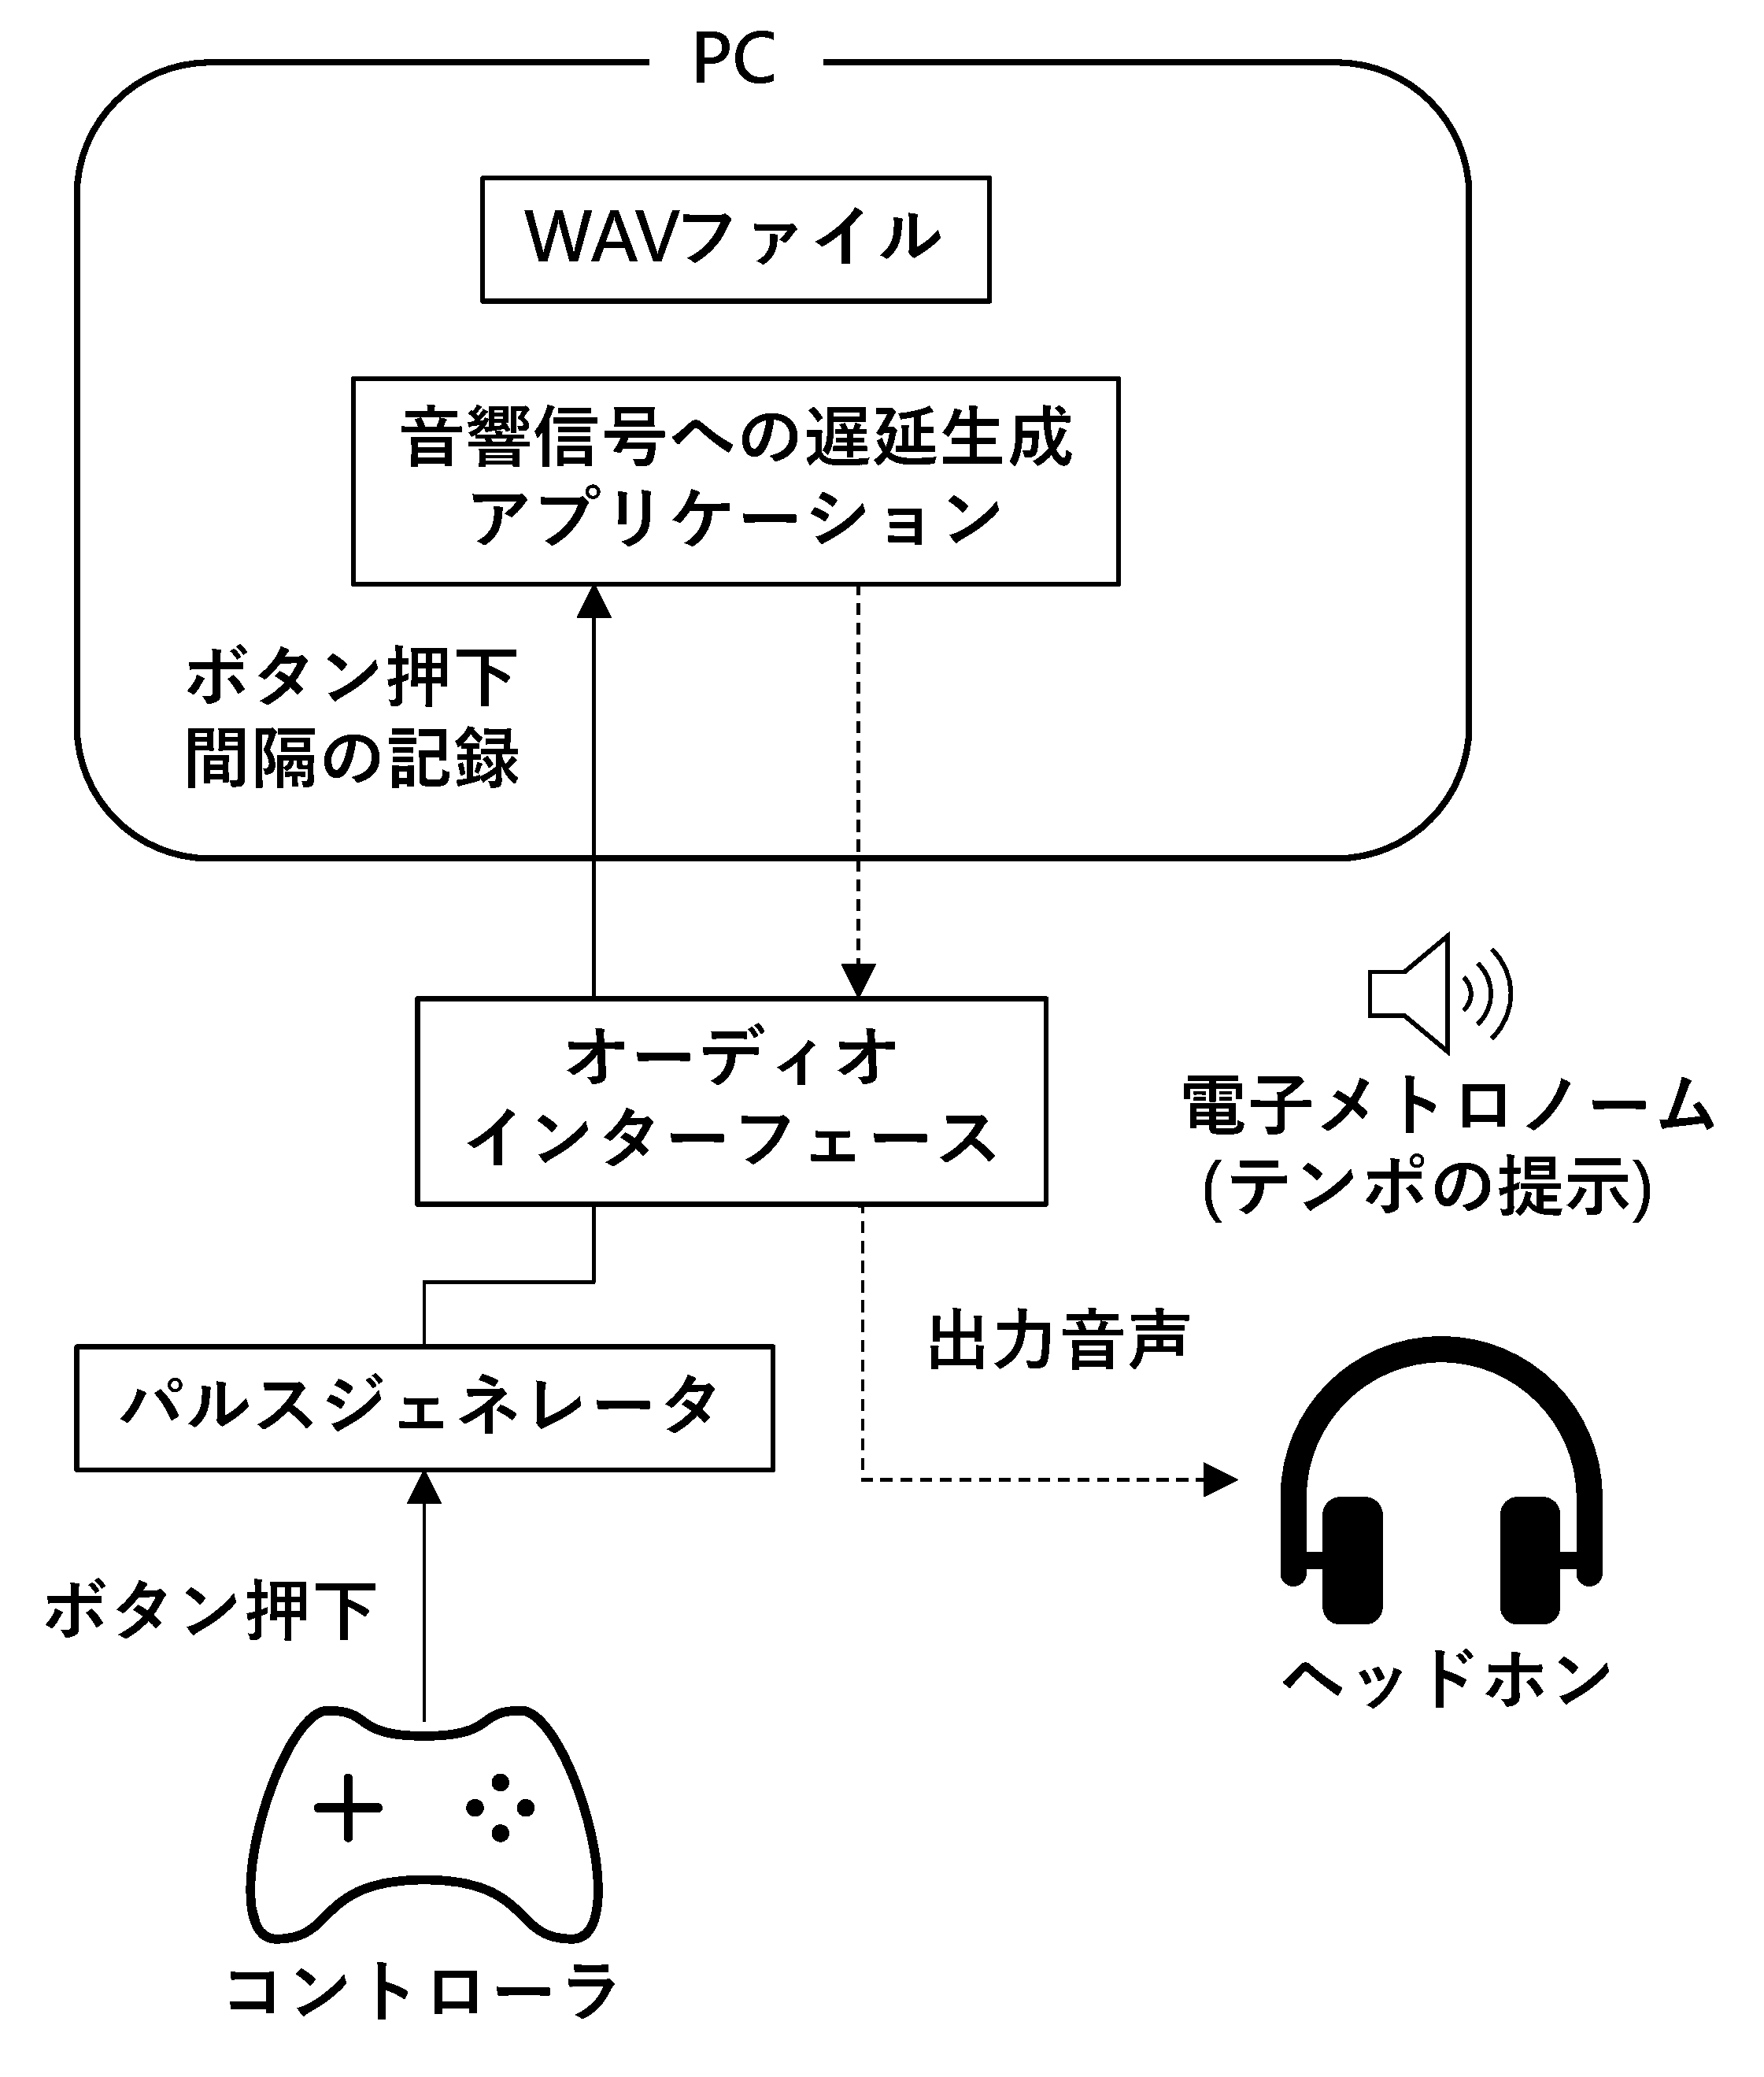
\includegraphics[scale=0.2]{figures/system_button_click.pdf}
  \caption{調査システムの構成}
  \label{fig:button-click-system}
\end{figure}
\begin{table}[tbp]
  \caption{使用機器}
  \label{table:device}
  \centering
  \begin{tabular}{lll}
    \hline
    使用機器 & 製造会社 & 製品名\\
    \hline \hline
    オーディオインターフェース & Focusrite & Scalett-Solo 3rd Generation\\
    コントローラー  & Nintendo & Super Famicom Controller\\
    開放型ヘッドホン & beyerdynamic & DT 990 PRO\\
    電子メトロノーム  & SEIKO  & DM71 Digital Metronome \\
    PC  & HP Inc. & 5 
    % パルスジェネレーター6 & 自作 & 
\\
    \hline
  \end{tabular}
\end{table}

手順1の後,被験者が装着しているヘッドホンから出力される音声の音量調節を行う.このとき,大きな遅延時間を提示すると調査で提示する全ての遅延時間について遅れていないと判断してしまう可能性が発話に関する調査で指摘されている\cite{Soturonn-takahashi}.
そのため,音量調節時に音響信号への遅延生成アプリケーションで指定する遅延時間は,一般的に遅延を感じないとされている10[ms]以下のものとする.また,音量調節時にヘッドホンから音声を出力している間,被験者には遅延のない音声を出力していると説明する.音量調節が完了したら,練習としてメトロノームの合図音に合わせて20回から40回ボタンを押下してもらい,実験の内容を理解させる.上記の手順によって記録されるボタンを押下する時間間隔及び,5章で説明する評価指標を用いて評価を行う.
\section{音響信号への遅延生成アプリケーション}
本研究で使用する音響信号への遅延生成アプリケーションは,Microsoft社が提供する統合開発環境であるVisual Studio 2022を用いてC++で開発する.このアプリケーションの表示例を図\ref{fig:app_kyakkann}に示す.
図\ref{fig:app_kyakkann}は,ボタン押し課題を開始し,アプリケーションのスタート直後の状態である.
被験者がボタンを押すと,押した時刻と直前に押した時刻からの経過時間[ms]が画面左側のエディットボックス内に書き込まれる.
実験が終了し,実験者が「ファイルへの出力」というプッシュボタンをクリックすると,実験者が指定したCSVファイルに結果が書き込まれる.
そして,開発したアプリケーションのソースコードを付録Bに掲載する.以下にアプリケーションの主な機能を示す.
\begin{enumerate}[leftmargin=*]
\item 任意の外部ファイルから複数の遅延時間を設定する機能
\item 実験者が画面上のコンボボックスで指定した時間だけ遅延させる機能(4.2.2項参照)
\item 被験者がボタンを押下する時間間隔を記録する機能(4.2.3項参照)
\item 被験者が押下するボタンの押下回数が実験者がアプリケーション上で指定した回数に到達したら合図音の出力を一時的に停止する機能
\item (3)で述べた記録とアプリケーション上での設定内容,被験者情報を外部ファイルに書き込む機能
\end{enumerate}
\begin{figure}[tb]
  \centering
  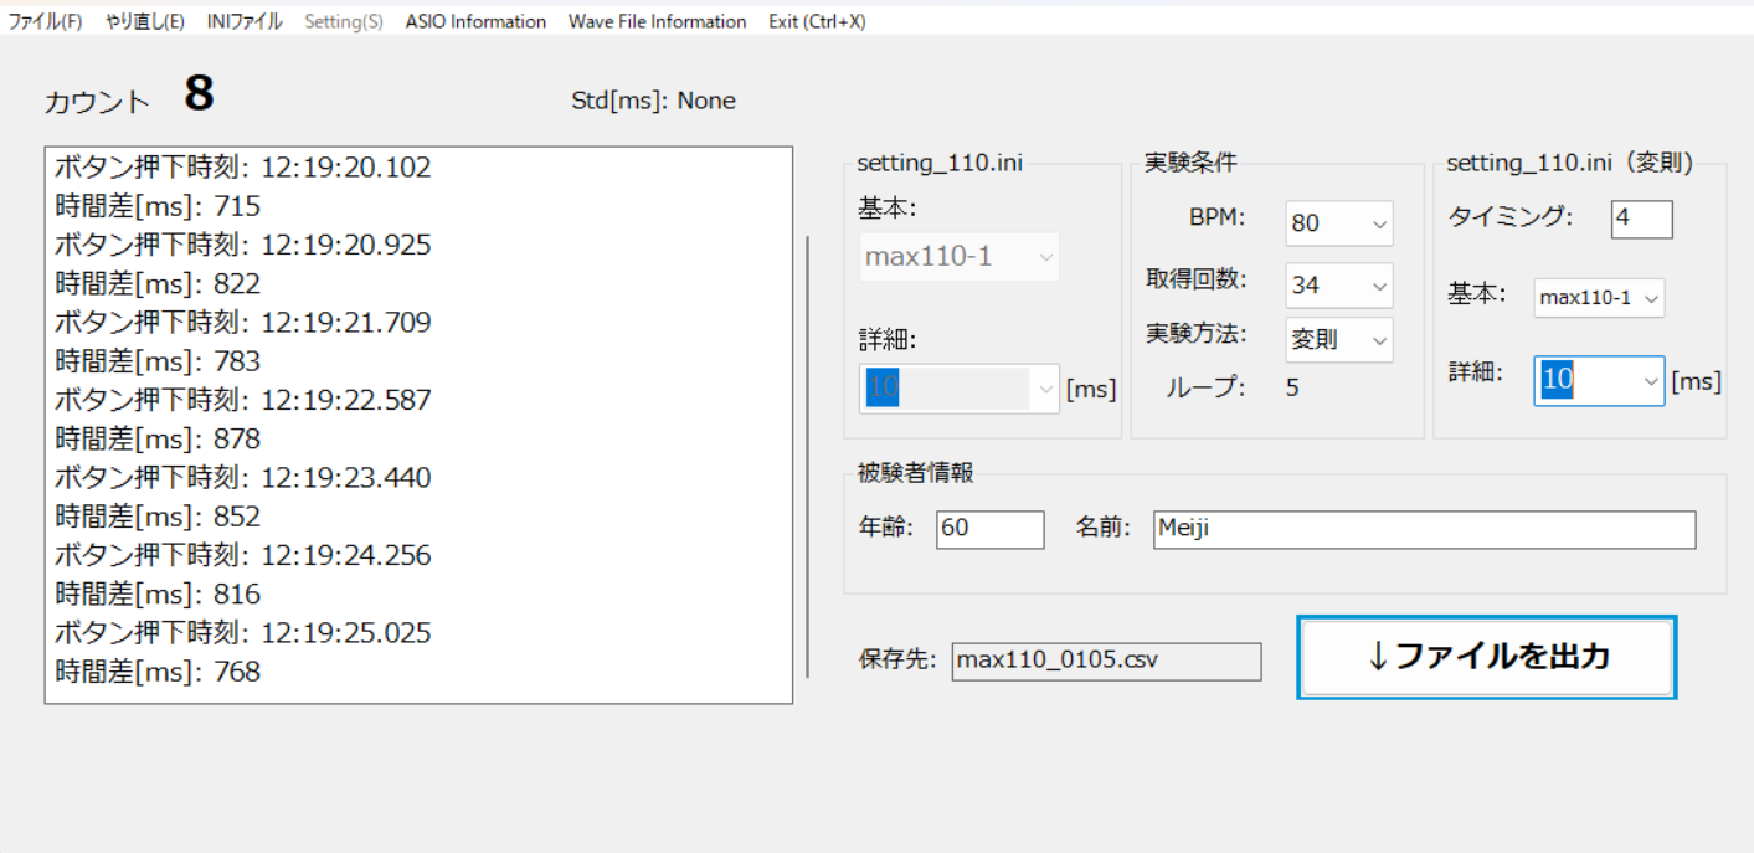
\includegraphics[scale=0.4]{figures/Apprication/App_kyakkann.pdf}
  \caption{実験開始直後の音響信号への遅延生成アプリケーションの画面}
  \label{fig:app_kyakkann}
\end{figure}
(1)はWindowsで主に使用されるINI(Initialization)ファイル形式を採用している.
遅延時間の一覧をINIファイルに予め設定し,アプリケーションから任意のINIファイルを選択し読み込むことで,
コンボボックスから遅延時間を選択する機能を実現している.
また,コンボボックスで選択された遅延時間をエディットボックスで指定したタイミングで発生させることも可能である.
さらに,選択された遅延時間に基づき遅延を発生させ,ボタンの押下回数が指定した回数に達し結果がファイルに書き込まれると,
コンボボックスの選択項目は自動的に次に移行する.
この機能により,ボタン押し課題はINIファイルの選択と結果を出力するプッシュボタンの押下のみで実施可能である.
\subsection{ASIOにおける音声の入出力}
本研究で開発するアプリケーションは,オーディオドライバにASIOを用いている.そこで,ASIOにおける音声の入出力方法について説明する.
ASIOではマルチバッファリングの切り替えを独自のコールバック関数で行う.独自のコールバック関数を用いることで,
バッファの切り替えはオーディオインターフェースによって行われるため,OSの影響を受けないという利点がある.
音声の入出力のシステムの動きを図\ref{fig:delay_theory}に示す.
入力で2つのバッファ,出力で2つのバッファを利用しそれぞれでダブルバッファリングを行う.
最初の入力バッファを入力バッファ1,次の入力バッファを入力バッファ2とし,最初の出力バッファを出力バッファ1,次の出力バッファを出力バッファ2とする.
それぞれ,音声の同時入出力が行われる前に0に初期化しておく.入力バッファ1に入力信号の格納が開始した時点から音声が出力される時点までの仕組みを以下に示す.
\begin{enumerate}[leftmargin=*]
\item はじめに入力バッファ1に入力信号が格納され,それと同時に出力バッファ1に格納されたデータの再生が始まる.しかし,この時点で出力バッファ1には録音データが格納されていないため,無音になる.
\item 入力バッファ1の格納可能な最大の許容量に達したとき,ASIOでコールバック関数が呼び出され,入力バッファ1と出力バッファ1がアプリケーションに受け渡される.それと同時に,入力バッファ2への録音データの格納が始まり,出力バッファ2の再生が始まる.ここでも,はじめは出力バッファ2にはまだ録音データが格納されていないため,無音となる.これと同時に,アプリケーション側ではコールバックにより入力バッファ1のデータを出力バッファ1にコピーする.
\item 入力バッファ2が格納可能な最大の許容量に達したとき,再びコールバック関数が呼び出され,出力バッファ1に格納された録音データの再生と入力バッファ1への入力信号の格納が開始する.
\item 手順2に戻る.
\end{enumerate}
以上を繰り返すことにより,音声の入出力を可能としている.しかし,このダブルバッファリングを用いた方法では,2バッファ分の遅延時間が常に発生する.
\subsection{任意の遅延時間後にボタン押下の合図音を再生させる機能}
任意の遅延時間が経過した後にWAVデータを再生させる機能は,ASIOにおける音声の同時入出力の方法に基づいて実装する.
ボタン押下の合図音の再生は,ボタン押下を検知した後に呼び出されるコールバック関数内で,保存されているWAVデータを入力バッファの代わりに出力バッファに転送することで行われる.
このWAVデータの出力バッファへの転送のタイミングを遅延時間ごとに調整することで,任意の遅延時間後にボタン押下の合図音を再生させる機能を実現させる.
また,図\ref{fig:delay_theory}のようにボタンの押下検知からWAVデータの再生までに少なくとも2つのバッファ分の遅延が生成されることになる.
バッファサイズが小さいほど,より高精度な遅延時間の設定が可能となる.
オーディオインターフェースのバッファサイズを$n$[points],サンプリング周波数を$f_{s}$[Hz],ASIOにおけるインターフェイスに固有の入力遅延を$i$[ms],ASIOにおけるインターフェイスの固有の出力遅延を$o$[ms],
% その他の遅延時間を$x$[ms],
所望の遅延時間を$d$[ms]とすると,遅延時間の生成は以下のような手順で実現される.
\begin{enumerate}[leftmargin=*]
  \item 初めに式\ref{eq:my_equation}に基づき,WAVデータのコピー時刻$T$を定義する.この時刻$T$は,ボタン押下の検出後,何回目のコールバック関数の呼び出し時にWAVデータをコピーするかを示す指標である.生成したい遅延時間$d$[ms]は,実験者がアプリケーション上で指定する.
\begin{equation}
T = \left\{ d - (i + o) \right\} \times n \times \left( \frac{f_s}{1000} \right) \label{eq:my_equation}
\end{equation}

  \item ボタンの押下を検知してから最初のコールバック関数呼び出し時を1回目として,$T-1$回目までは,入力バッファに格納されているデータを出力バッファにコピーする.このとき,入力バッファには0が格納されているため無音となる.
  \item ボタンの押下を検知してから$T$回目のコールバック関数呼び出し時になったら,入力バッファに格納されているデータの代わりにWAVデータを出力バッファにコピーしていく.
\end{enumerate}
上記の手順を踏むことにより,任意の遅延時間の生成を実現する.
\begin{figure}[h]
  \centering
  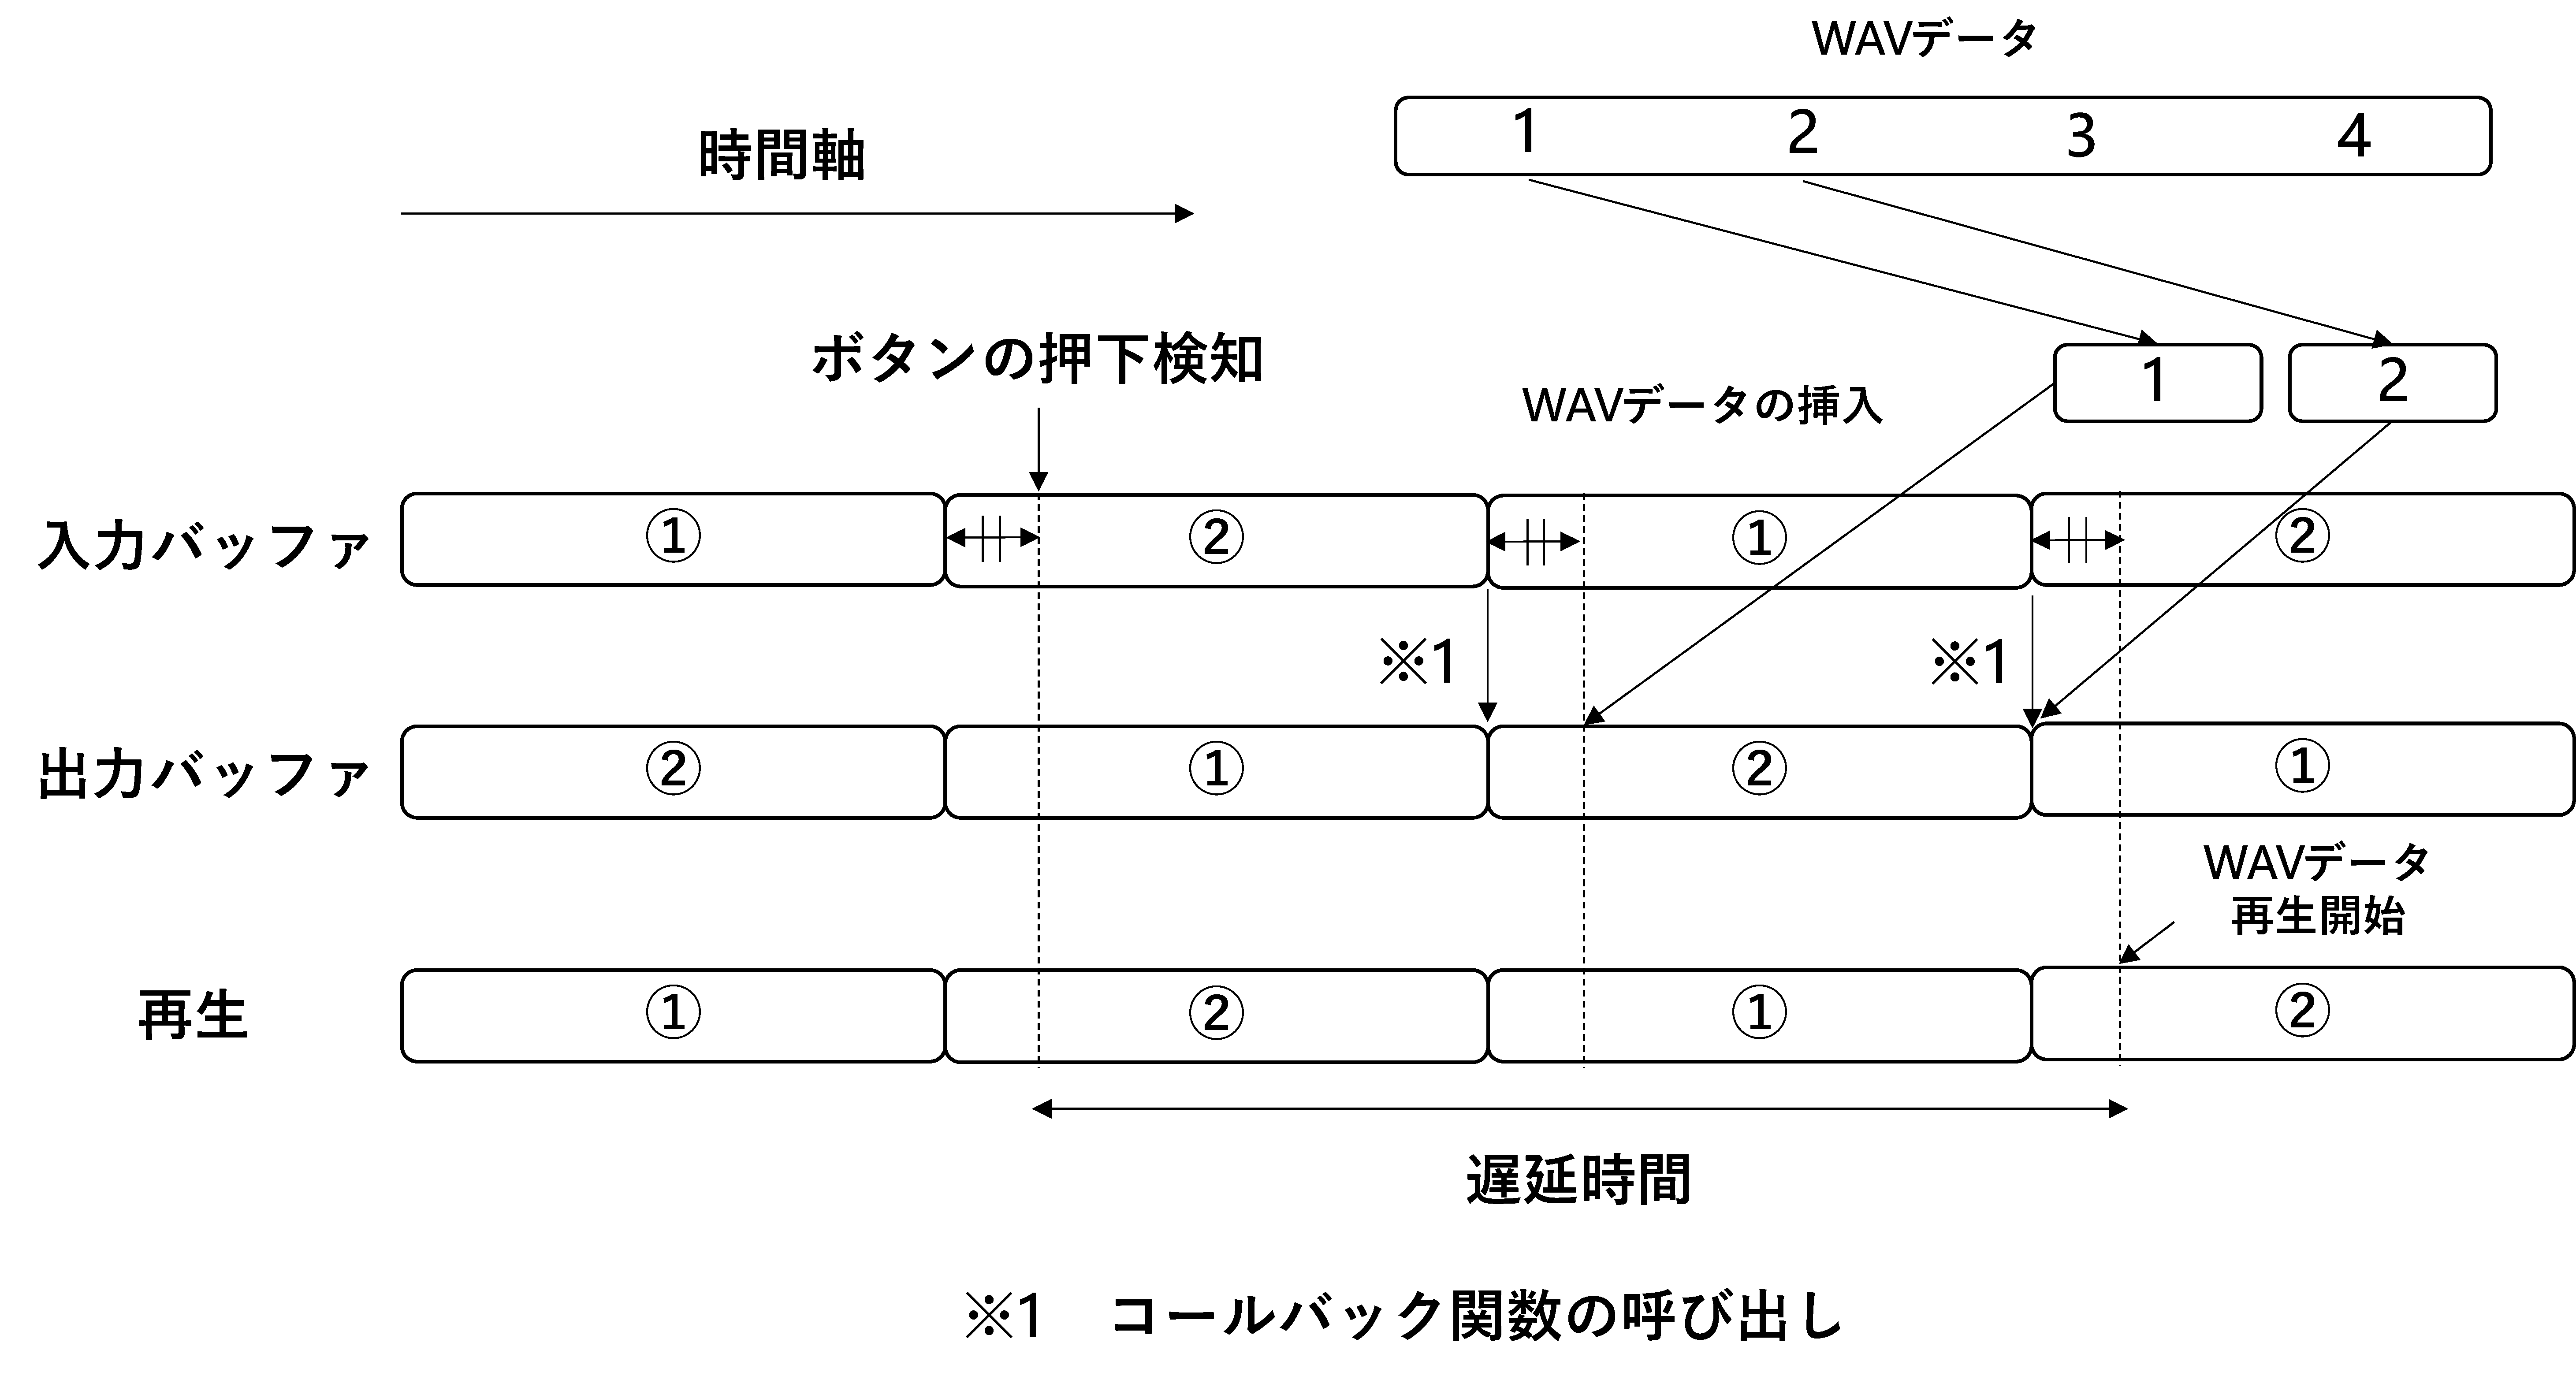
\includegraphics[scale=0.12]{figures/System/Delay_theory.pdf}
  \caption{遅延時間の生成原理}
  \label{fig:delay_theory}
\end{figure}
\subsection{ボタンの押下時間間隔を記録する機能}
ボタンの押下時間間隔を記録する機能は,ボタンを押下するごとに,ボタンの押下と押下の間の時間を計測する.
例外として,1回目のボタンの押下時間間隔は記録しないように設定する.
押下時間間隔の取得には,C++の標準ライブラリであるstd::chronoを使用する.
std::chronoは,C++11以降で使用可能な時間に関する操作を提供するライブラリである.
以下に押下と押下の間の時間を計測するための手順を示す.
\begin{enumerate}[leftmargin=*]
\item ボタン押下を検知したら,関数std::chrono::system\_clock::now()を使用してエポック(1970年1月1日0時0分0秒 UTC)からの経過時間を取得し,用意した変数Aに代入する.
\item 再びボタンの押下を検知したら,変数Aを別の変数Bに代入し,変数Aに手順1と同様の方法でエポックからの経過時間を取得し,代入する.
\item ボタンの押下が2回目以降であれば,手順2の後に変数Bと変数Aの差を計算し,変数Cに代入する.
\item 関数std::chrono::duration\_cast\textless std::chrono::milliseconds\textgreater()によって変数Cをミリ秒単位の時間に変換する.
\item 手順3で変換した変数Cを随時,動的な配列に追加していくことで全てのボタンの押下時間間隔を記録する.
\end{enumerate}
\section{生成する遅延時間の正確性の調査}
\subsection{遅延時間の測定方法}
アプリケーションによって生成された遅延時間の正確性を検証する目的で,遅延時間の測定を行う.
図\ref{fig:delay_check}に遅延時間の測定の接続図を示す.
測定手順は以下の通りである.
\begin{figure}[tb]
  \centering
  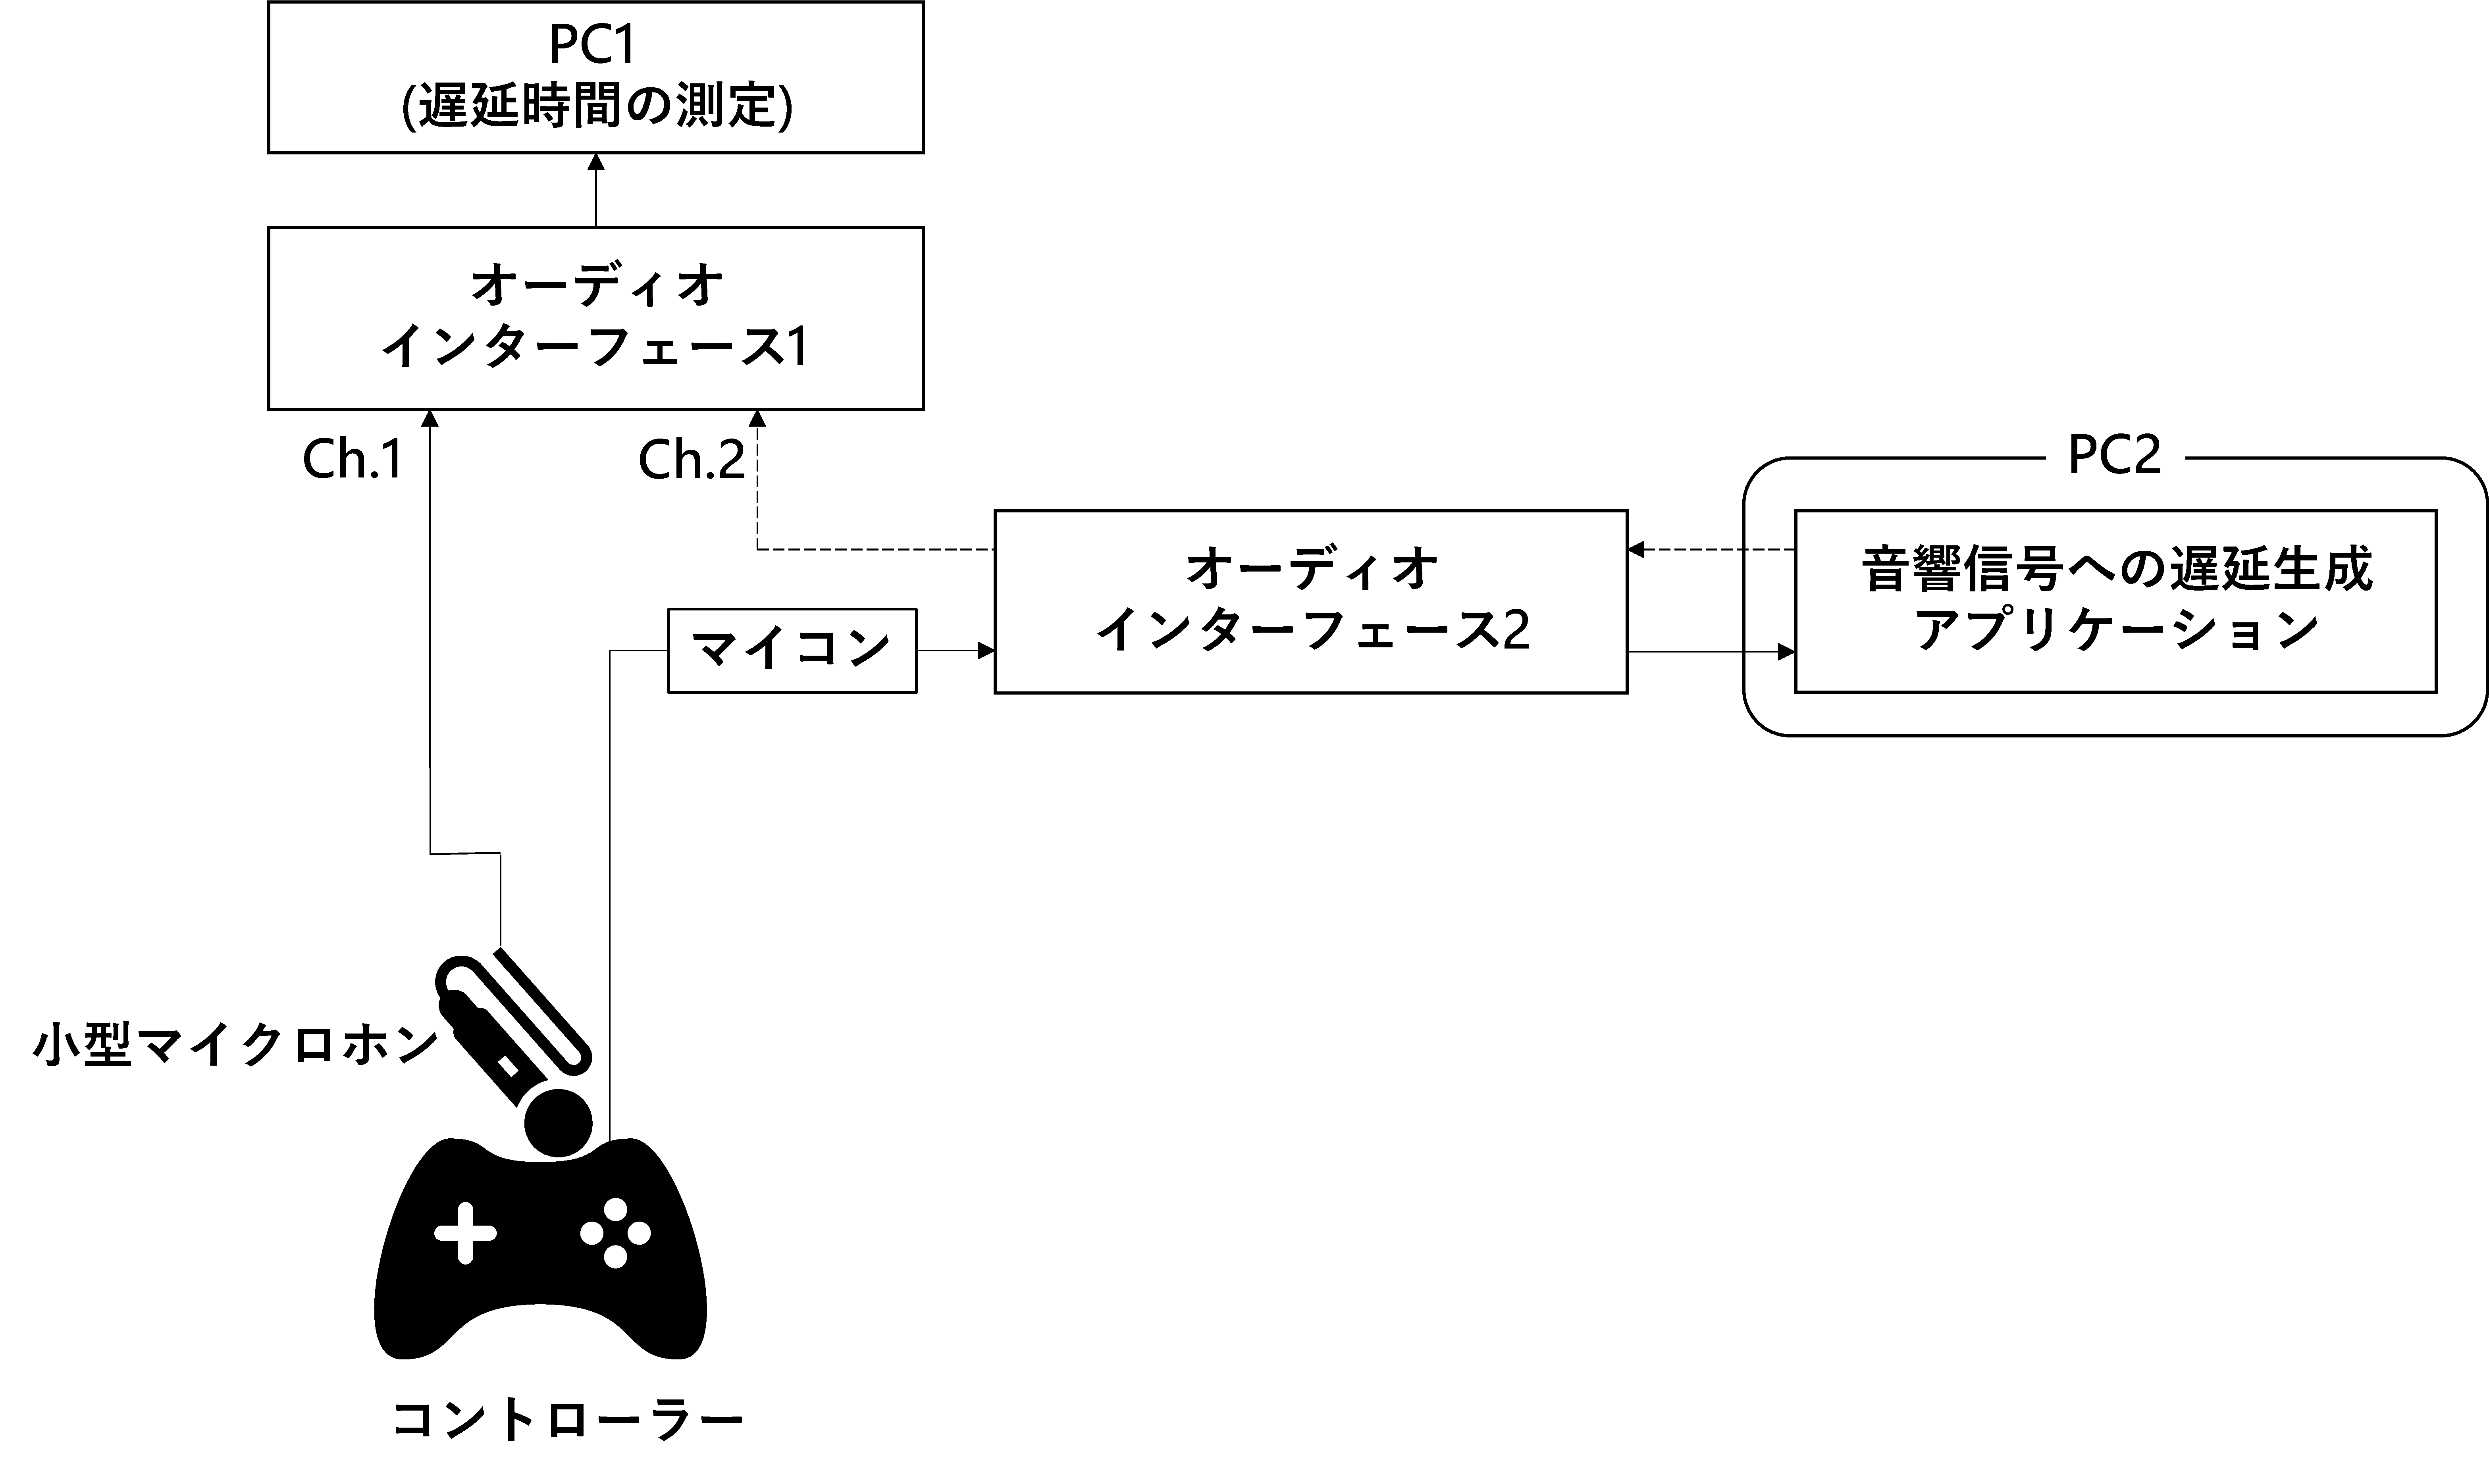
\includegraphics[scale=0.1]{figures/DelayCheck/DelayCheck_EX.pdf}
  \caption{遅延時間測定のための接続図}
  \label{fig:delay_check}
\end{figure}
\begin{enumerate}[leftmargin=*]
  \item 測定システムを図\ref{fig:delay_check}に示された構成で用意する.
  \item 遅延時間測定のためのプログラムと遅延時間生成アプリケーションが起動してから十分に時間が経過した状態で,実験者はボタンを押下する.
  \item 図\ref{fig:super_famicom}のような小型マイクロホンを取り付けたコントローラーから取得した音をオーディオインターフェース1のチャンネル1へと入力する.
  \item コントローラーのボタンを押下することで,遅延生成アプリケーションを介して出力される音声をオーディオインターフェース1のチャンネル2へ入力する.
  \item チャンネル1に入力された信号の開始点から1000点目の点から6000点目の点の信号の振幅の平均と標準偏差を求める.
  チャンネル1において,平均 + 2 × 標準偏差を超えた点を検出し,チャンネル1に入力された信号(小型マイクロホンから取得した音響信号)の開始点とする.
  \item チャンネル2においても同様に,平均 + 2 × 標準偏差を超えた点を検出し,
  これをチャンネル2における信号(アプリケーションによって生成された音響信号)の開始点とする.
  \item それぞれの開始点の時間差を計算し,これを遅延時間[ms]として算出する.
\end{enumerate}
\begin{figure}[bt]
  \centering
  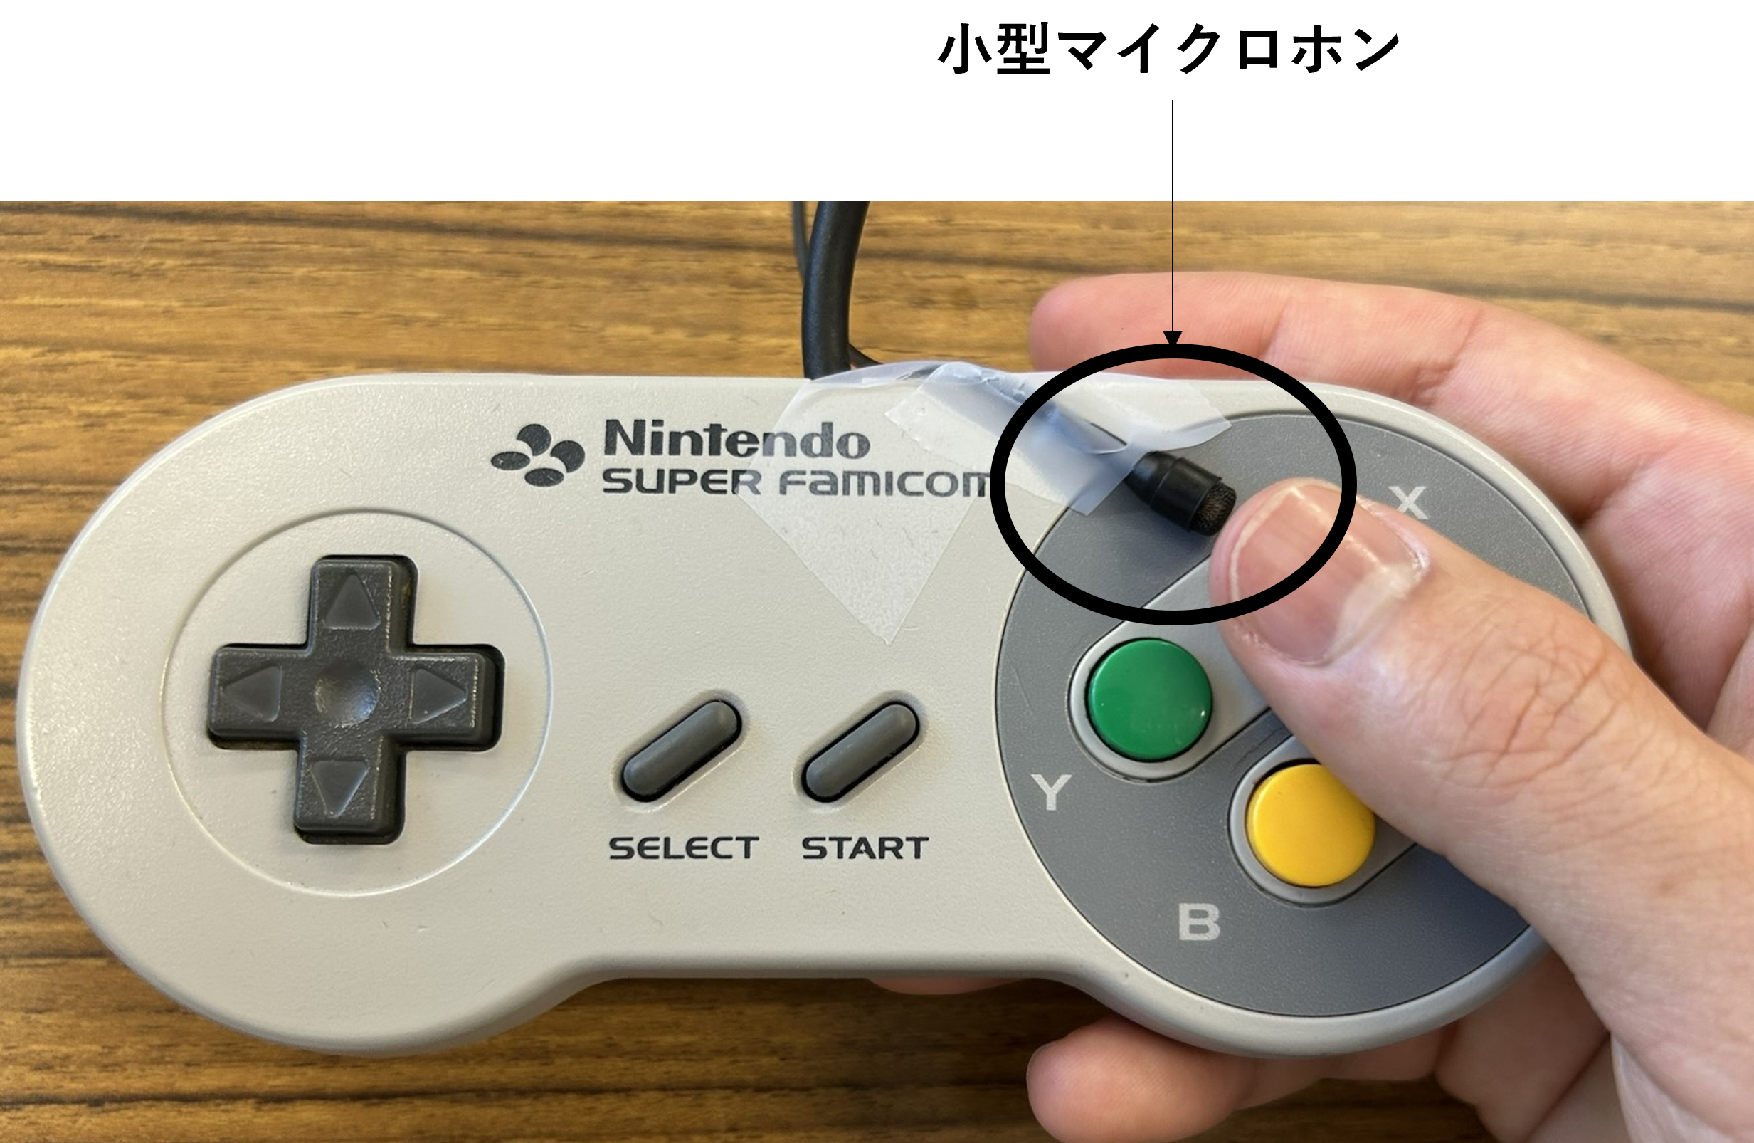
\includegraphics[scale=0.5]{figures/DelayCheck/SuperFamicom_delayCheck.png}
  \caption{小型マイクロホンを装着しているコントローラー}
  \label{fig:super_famicom}
\end{figure}
システムの動作確認は,次の方法で実施した.アプリケーションの遅延時間の設定値を10[ms]に設定し,生成される遅延時間を計測した.
このプロセスでは,PC上で他アプリケーションによるCPU占有が生じてもシステムが正常に機能するかを検証するため,遅延時間生成用PCの全CPUコアを利用して重い計算を実行し,
CPU使用率を100%に保ち,この状態と通常のCPU負荷がない状態の両方で遅延時間を測定した.
CPU使用率を100%にするプログラムと遅延時間測定プログラムは,付録Bに掲載している.
この測定は合計10回行い,遅延時間の理論値と実測値の差の絶対値の平均および実測値の標準偏差を算出した.
使用した機器の詳細は表\ref{table:device_delay_check}に示す.
また,設定するバッファサイズをオーディオインターフェースで設定可能な最小のバッファサイズである16とし,
遅延時間を10-40[ms]の範囲では5[ms]ずつ,
50-150[ms]の範囲では20[ms]ずつ変化させ,それぞれの場合において生成された遅延時間を4.3.1項で説明した方法で測定する.
% \subsection{測定条件}
\begin{table}[tbp]
  \caption{測定に使用した機器}
  \label{table:device_delay_check}
  \centering
  \begin{tabular}{lccc}
    \hline
    実験装置 & 製造会社 & 製品名\\
    \hline \hline
    オーディオインターフェース1  & Roland & Duo-Capture EX\\
    オーディオインターフェース2  & Forcusrite & Scarett-solo 3rd Generation\\
    遅延時間生成用のPC  & HP & HP ProBook 450 G7\\
    遅延時間測定用のPC  & HP & pavilion\\
    マイクロホン  & DPA Microphones & IMK-SC4060
\\
    \hline
  \end{tabular}
\end{table}

\subsection{測定結果}
表\ref{table:delay_check_result}に測定結果を示す.
表\ref{table:delay_check_result}よりCPU利用率が平常時においては,理論値の誤差と実測値の差が小さいことから,アプリケーションの正常な動作が確認された.
一方で,CPU利用率が100%の状態では,理論値と実測値の差および実測値の標準偏差が著しく増加することが確認された.
これは,本研究で開発されたアプリケーションが,CPU利用率が100%の際には正常に機能しないことを示している.
したがって,本研究で開発されたアプリケーションを用いてボタン押し課題を実施する際には,CPU利用率が100%に至らないよう注意が必要であり,
実験を行う研究者は,他のアプリケーションを終了させる等の措置を講じ,CPU利用率が100%にならないように慎重に実験を進める必要がある.
\begin{table}[tbp]
  \caption{測定結果}
  \label{table:delay_check_result}
  \centering
  \begin{tabular}{ccccc}
    \hline
    \begin{tabular}{c}
      CPU \\ 利用率
    \end{tabular}
    & 
    \begin{tabular}{c}
      オーディオ入出力の \\ バッファサイズ
    \end{tabular}
    &
    \begin{tabular}{c}
      理論値と実測値の \\ 差の絶対値の平均[ms]
    \end{tabular}
    & 
    \begin{tabular}{c}
      実測値の \\ 標準偏差[ms]
    \end{tabular}
     \\
    \hline \hline
    平常時  & 16 & 0.129 & 1.23\\
    100[%]時  & 16 & 5.08 & 4.93\\
    \hline
  \end{tabular}
\end{table}
